\documentclass[]{article}
\usepackage{mathtools}
\usepackage[pdftex]{graphicx}	
\usepackage{amsmath,amsfonts,amsthm}	
\usepackage{tikz}
\usepackage{listings}
\usetikzlibrary{chains, positioning}
\newtheorem{theorem}{Twierdzenie}[section]
\newtheorem{lemma}[theorem]{Lemma}
\newtheorem{proposition}[theorem]{Proposition}
\newtheorem{corollary}[theorem]{Corollary}
\usepackage{sidecap}
\usepackage{polski}
\usepackage[utf8]{inputenc}
\usepackage[T1]{fontenc}
\usepackage{caption} 
\captionsetup[table]{skip=10pt}
\usepackage{subfigure}
\sidecaptionvpos{figure}{t}
\usetikzlibrary{calc,arrows}
\usepackage{slashbox}
\usetikzlibrary{chains, positioning}

\theoremstyle{definition}
\newtheorem{definition}{Definicja}[section]
\usepackage{color}
\usepackage{hyperref}
\hypersetup{
	colorlinks=true,
	linkcolor=black,
	urlcolor=red,
	linktoc=all
}

\lstset{
	language=Python,
	basicstyle=\ttfamily\small,
	numberstyle=\footnotesize,
	%numbers=left,
	%backgroundcolor=\color{gray!10},
	frame=single,
	tabsize=2,
	rulecolor=\color{black!30},
	title=\lstname,
	escapeinside={\%*}{*)},
	breaklines=true,
	breakatwhitespace=true,
	framextopmargin=2pt,
	framexbottommargin=2pt,
	inputencoding=utf8,
	extendedchars=true,
	literate={ą}{{\k a}}1 {ę}{{\k e}}1,} %{ś}{{\'s}}1,


%\usepackage{xcolor}
%\colorlet{RED}{black} % don't color running headers
%\colorlet{BLUE}{black}
%\usepackage[titles]{tocloft}


%opening
\title{}
\author{Rafal Skrzypiec}
\date{}
\begin{document}

\maketitle
\tableofcontents

\newpage

Co poprawić z obecnego tekstu:
\begin{itemize}
	\item w całym tekście zacząć dodawać cytowania
	\item Twierdzeneie Cybenki	
	\begin{itemize}
			\item  bardziej dokładnie i logicznie przeprowadzić dowód twierdzenia
			\item  opisać wizualne przedstawienie twierdzenia i stworzyć rysunki z polskimi podpisami				
	\end{itemize}
	\item uporządkowaąć kolejność podrozdziałów nt. metodologii
\end{itemize}



\newpage


\section{Wstęp}
\subsection{Fizyka zagadnienia i cel pracy}
\subsection{Sieci neuronowe, wysokopoziomwy opis, zastosowania - regresja i klasyfikacja}

\newpage

\section{Sieci Neuronowe}
\subsection{Historia sieci - perceptron, biologia}
\subsection{Funkcje aktywacji, dlaczego sigmoidy}
%[\color{red}Funkcje aktywacji, dlaczego sigmoidy]
Funckja aktywacji to funkcja, która działa na każdy neuron w sieci neuronowej, jako argument przyjmuje sumę iloczynów wartości neuronów z warstwy poprzedzającej i odpowiadających im wag. Każda z warstw sieci neuronowej może mieć zdefiniowaną inną funckję aktywacji.

Perceptron, który był inspiracją powstania sieci neuronowcyh został skonstruowany jako uproszczony model biologicznego neuronu. W neurobiologii, neuron jest 
komórką, która odbiera, przetwarza i przesyła informacje wykorzystując elektryczne i chemiczne sygnały. Neurony połączone są ze sobą przez synapsy, jeden neuron może otrzymywać informacje od wielu komórek nerwowych. Jeśli suma sygnałów elektrycznych z wejściowych synaps przekroczy pewien próg, wtedy neuron transmituje dalej sygnał elektryczny. Perceptron naśladował ten mechanizm stosując przedstawioną w lewym górnym rogu na Rys.~\ref{fig:activations} funckję Heaviside'a jako funkcję aktywacji. Funkcja przyjmuję wartość jeden jeśli suma wartości wejściowych jest większa od zera, w innym przypadku funkcja przyjmuje wartość zero i neuron nie propaguje sygnału. Perceptron jest najprostszym przykładem sieci neuronowej.

Wyniki badań przeprowadzonych przez [publikacja, publikacja] pokazały, że wśród pożądanych cech funkcji aktywacji znajdują się atrybuty, których funkcja Heaviside'a nie posiada, z tego powodu nie jest w praktyce często stosowana.

Koniecznym wymaganiem jest nieliniowość stosowanej funkcji, jest to cecha, która pozwala sieci neuronowej odwzorować nieliniowe zależności [LeCun, Cybenko?, Hornik]. Jedynym wyjątkiem od reguły jest stosowanie w problemach regresyjnych funkcji tożsamościowej w ostatniej warstwie wyjściowej. Dobrze gdy funkcja posiada ciągłą pochodną, pozwala to na stosowanie metod optymizacji opartych o obliczanie gradientu. Tu wyjątkiem jest stosowana poprawiona jednostka liniowa (ReLU), również przedstawiona na Rys.~\ref{fig:activations}. Zakładając, że w zerze jej gradient równy jest zero możemy skorzystać z jej wielu zalet. Wśród nich wymienia się dokładniejsze odwzorowanie obserwowanego w neurobiologii zjawiska -- tylko neurony, które otrzymały odpowiednio silny sygnał są aktywowane. Brak podatności na przeuczenie, podczas inicjalizacji sieci losowymi wagami, tylko około 50\% ukrytych neuronów jest aktywowanych. Brak problemu znikającego gradientu uniemożliwiającego uczenie, w porównaniu do sigmoidy, u której wysyca się on w obu kierunkach. Jest to również funkcja często wykorzystywana w metodach głębokiego uczenia. W warstwach splotowych sieci która służy do rozpoznawania obrazów wykorzystamy ReLU poszukując atrybutów, które nie zmieniają się podczas jej użycia.
%
\begin{figure}[h!]
	\centering
	\includegraphics[width=\linewidth]{activations14_12}
	\caption{Kilka przykładów często stosowanych funkcji aktywacji.}
	\label{fig:activations}
\end{figure}
%
%
\subsubsection{Funkcje sigmoidalne}
%
Częstym wyborem funkcji aktywacji są funkcje sigmiodalne. Jest to grupa monotonicznie rosnących funkcji, których zbiór wartości jest ograniczony przez asymptoty o skończonych wartościach, do których wartość funkcji dąży w $\pm \infty$ [lecun98]. Jednym z najczęściej wykorzystywanych przykładów funkcji sigmoidalnych jest sigmoida zdefiniowana równaniem
%
\begin{equation}
\sigma(x) = \frac{1}{1+e^{-x}}.
\end{equation}
%
Sigmoida jest różniczkowalna w każdym punkcie co pozwala używać podczas procesu uczenia metod optymizacji wykorzysujących gradient. Ponadto pochodna względem argumentu $x$ wyraża się prostą relacją
%
\begin{equation}
\frac{d}{dx} \sigma(x)= \sigma(x)\left(1 - \sigma(x)\right).
\end{equation}
%
%
\begin{figure}[h!]
	\centering
	\includegraphics[width=\linewidth]{sigmoid14_8}
	\caption{Przykład funkcji sigmoidalnej - sigmoida, $\sigma(x) = \frac{1}{1+e^{-x}}$}
\end{figure} 

Innym przykładem często wykorzystywanej w sztucznych sieciach neuronowych funkcji sigmoidalnej jest tangens hyperboliczny (prawy dolny róg Rys. \ref{fig:activations}). Wzór tej funkcji możemy wyrazić korzystając z definicji sigmoidy
\begin{equation}
\tanh(x) = 2\sigma(2x)-1
\end{equation}
%
Jedną z zalet tej funkcji jest symetryczność względem początku układu współrzędnych.
%
\subsubsection{Interpretacja probabilistyczna sigmoidy}
%
Zastosowanie sigmoidy jako funkcji aktywacji naturalnie wynika z postaci prawdopodobieństwa a posteriori w Bayesowskim podejściu do problemu klasyfikacji dwóch klas.
%
Rozważmy sztuczną sieć neuronową z jedną warstwą ukrytą oraz funkcję dyskryminacyjną $y(\mathbf{x})$ taką, że wektor $\mathbf{x}$ jest przypisany do klasy $C_1$ jeśli $y(\mathbf{x}) > 0$ i do klasy $C_2$ jeśli $y(\mathbf{x}) < 0$.
\\
W najprostszej, liniowej formie funkcja może być zapisana jako:
%
\begin{equation}
y(\mathbf{x}) = \mathbf{w}^\mathsf{T} \mathbf{x} + b_0.
%\label{sum}
\end{equation}
%
Wektor $\mathbf{w}$, to $d$-wymiarowy wektor wag, natomiast parametr $b_0$ to bias.
%
Rozważmy funkcję $g(\cdot)$ nazywaną dalej funkcją aktywacji, która jako argument przyjmuje jako argument sumę z równania (\ref{suma}):
%
\begin{equation}
y = g\left(\mathbf{w}^\mathsf{T} \mathbf{x} + b_0 \right)
\label{suma}
\end{equation}
%
\def\layersep{2.5cm}

\begin{SCfigure}
	\centering
	
	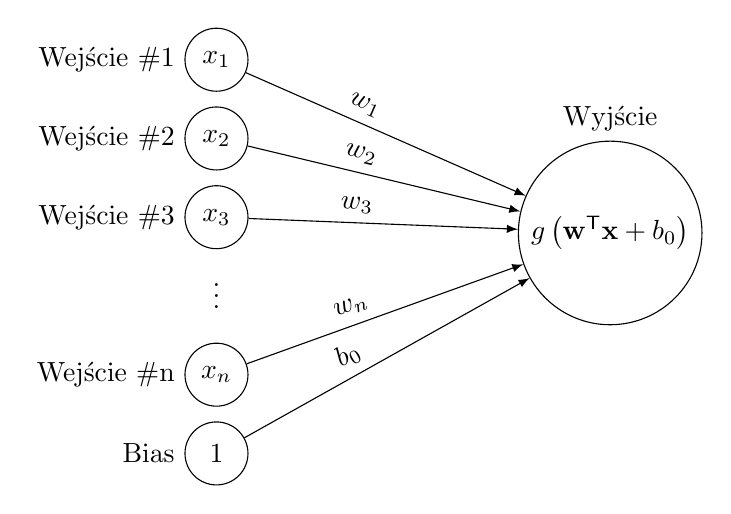
\begin{tikzpicture}
	[   cnode/.style={draw=black,draw=black,fill=#1,minimum width=8mm,circle},
	]
	\tikzset{normal arrow/.style={draw,-latex}}
	\node[cnode=white,label=90:Wyjście] (s) at (5,-3.2) {$ g\left(\mathbf{w}^\mathsf{T} \mathbf{x} + b_0 \right)$};
	\node at (0,-3.9) {$\vdots$};
	
	\node[cnode=white,label=180:Bias] (x-5) at (0,-6) {1};
	
	\foreach \x in {1,...,4}
	{
		\pgfmathparse{\x<4 ? \x : "n"}	   
		\ifnum \x = 4
		\node[cnode=white,label=180:Wejście \#n] (x-\x) at (0,{-1*\x-div(\x,4)}) {$x_{n}$};
		
		\else
		
		\node[cnode=white,label=180:Wejście \#\pgfmathresult] (x-\x) at (0,{-1*\x-div(\x,4)}) {$x_{\x}$};
		\fi
		\path[normal arrow] (x-\x) -- node[above,sloped,pos=0.4] {$w_{\pgfmathresult}$} (s);
	}
	\path[normal arrow] (x-5) -- node[above,sloped,pos=0.4] {$b_0$} (s);	
	\end{tikzpicture}
	\caption{ Reprezentacja funkcji dyskryminacyjnej $y(x)$ w postaci diagramu sieci neuronowej, mającej $n$ wejść, parametr bias i jedno wyjście.  }
\end{SCfigure}
%
Załóżmy, że funkcja rozkładu prawdopodobieństwa danych pod warunkiem klasy $C_k$ zadane jest przez wielowymiarowy rozkład normalny z równymi macierzami kowariancji $ \Sigma_1 = \Sigma_2 = \Sigma$
%
\begin{equation}
p(x|C_k) = \frac{1}{\left(2 \pi\right)^{\frac{d}{2}} \left| \Sigma \right|^{\frac{1}{2}}} \exp \left[ -\frac{1}{2} \left(\mathbf{x} - \mathbf{\mu}_k\right)^\mathsf{T} \Sigma^{-1} \left(\mathbf{x} - \mathbf{\mu}_k \right) \right].
\end{equation}
%
Prawdopodobieństwo a posteriori klasy $C_1$ można zapisać używając twierdzenia Bayesa:
%
\begin{eqnarray}
p(C_1 | \mathbf{x}) &=& \frac{p(\mathbf{x}|C_1) p(C_1)}{ p(\mathbf{x}|C_1) p(C_1) + p(\mathbf{x}|C_2)p(C_2)} \nonumber\\
&=& \frac{1}{1 + \frac{p(\mathbf{x}|C_2)p(C_2)}{p(\mathbf{x}|C_1)p(C_1)}} \nonumber\\ 
&=& \frac{1}{1 + \exp(-a)},
\end{eqnarray}
%
gdzie
%
\begin{eqnarray}
a &=& \ln \frac{p(\mathbf{x}|C_1)p(C_1)}{p(\mathbf{x}|C_2)p(C_2)} \nonumber \\
&=& \left( \mu_1 - \mu_2 \right)^{\mathsf{T}} \Sigma^{-1} \mathbf{x}  - \frac{1}{2} \mu_1^\mathsf{T}\mu_1 + \frac{1}{2} \mu_2^\mathsf{T} \Sigma^{-1} \mu_2 + \ln \frac{p(C_1)}{p(C_2)},
\end{eqnarray}
%
pamiętając o tym, że macierz kowariancji jest symetryczna otrzymujemy
%
\begin{subequations}
	\begin{align}
	\mathbf{x} &= \Sigma^{-1} \left(\mu_1 - \mu_2\right)\\
	b_0 &= - \frac{1}{2} \mu_1^\mathsf{T}\mu_1 + \frac{1}{2} \mu_2^\mathsf{T} \Sigma^{-1} \mu_2 + \ln \frac{p(C_1)}{p(C_2)}
	\end{align}
\end{subequations}
%
Zatem widzimy, że użycie funkcji aktywacji w postaci sigmoidy pozwala nie tylko dokonać decyzji klasyfikacji ale również interpretować wynik funkcji dyskryminacyjnej jako prawdopodobieństwa a posteriori.
%


\subsection{Opis algorytmu uczenia prostej sieci}

\subsubsection{Dane}

Zbiór danych treningowych zawiera $m$ jednowymiarowych próbek zadanych przez wektory $X \in \mathbb{R}^{1\times m}$ i odpowiadające im wyniki $Y\in \mathbb{R}^{1\times m}$.



\subsubsection{Parametry}

Sieć ma dwie warstwy: 1) ukryta, zawierająca $L$ neuronów i 2) wyjściowa, składająca się z $1$ neuronu. Warstwy są zdefiniowane przez:

1. parametry wartstwy ukrytej, które odwzorowują $1$-wymiarowe wektory wejściowe w aktywacje $L$ neuronów:
macierz wag $W^h\in\mathbb{R}^{L\times 1	}$ i wektor parametru bias $b^h\in\mathbb{R}^{L\times 1}$,

2. parametry wartstwy wyjściowe, które odwzorowują $L$-wymiarowy wektor aktywacji neuronów ukrytych w jeden neuron wartstwy wyjściowej:
macierz wag $W^o\in{1\times L}$ i wektor bias $b^o\in\mathbb{R}^{1\times 1}$.


\subsubsection{Propagacja sygnału}

Wejście każdego neuronu w warstwie ukrytej jest iloczynem danych wejściowych i odpowiadającej im wagi plus parametr bias. Na przykład dla $i$-tego przykładu danych wejściowych, w $l$-tym neuronie mamy

\begin{equation}
{a^h}^{(i)}_l = {W^h}_{l}x^{(i)} + {b^h}_l
\end{equation}

%Wejście wszystkich neuronów dla wszystkich przykładów może być wyrażone przez macierze, używając mnożenia macierzy oraz broadcastingu (możliwości dodania wektora kolumnowego do wszystkich wektorów kolumnowych w macierzy) mamy

%\begin{equation}
%{a^h} = W^h\cdot x + b^h
%\end{equation}
%Co w Pythonie można zapisać jako $ah = W.dot(x) + b$


Funkcją aktywacyjną neuronów jest sigmoida $\sigma(a) = \frac{1}{1+e^{-a}}$, jako argument przyjmuje ona wejście neuronów:

\begin{equation}
{h^h}^{(i)}_l=\sigma({a^h}^{(i)}_l)
\end{equation}


Neuron warstwy wyjściowej zawiera sumę iloczynów aktywacji neuronów i odpowiadających im wag plus parametr bias. Dla $i$-tego przykładu mamy

\begin{equation}
\begin{split}
{a^o}^{(i)} &= \sum_{l} {W^o}_l{h^h}^{(i)}_l + {b^o} \\
& = \sum_{l} {W^o}_l\sigma({a^h}^{(i)}_l) + {b^o} \\
& = \sum_{l} {W^o}_l\sigma({W^h}_{l}x^{(i)} + {b^h}_l) + {b^o}
\end{split}
\end{equation}

Jako funkcja straty zostanie wykorzystany błąd średniokwadratowy

\begin{equation}
\begin{split}
J^{(i)}(\Theta) &= \frac{1}{2} \left( y^{(i)}- a^{o{(i)}}  \right)  ^2 \\
J(\Theta) &= \frac{1}{m}\sum_{i=1}^m J^{(i)}(\Theta)= \frac{1}{2m}\sum_{i=1}^m \left( y^{(i)}- a^{o{(i)}}  \right)  ^2  .
\end{split}
\end{equation}


\subsubsection{Propagacja wsteczna}


Użycie reguły łańcuchowej umożliwia obliczenie gradientu funkcji straty względem parametrów sieci neuronowej.

Na początku policzmy gradient względem wyniku wartstwy wyjściowej.



\begin{equation}
\frac{\partial J}{\partial {a^o}^{(i)}} = \frac{1}{m} \left( y^{(i)}- a^{o{(i)}}  \right),
\end{equation}

następnie policzmy gradient wyjścia neuronów ukrytych:

\begin{equation}
\frac{\partial J}{\partial {h^h}^{(i)}_l} = \frac{\partial J}{\partial {a^o}^{(i)}} \frac{\partial {a^o}^{(i)}}{\partial {h^h}^{(i)}_l} =  \frac{\partial J}{\partial {a^o}^{(i)}} {W^o}_{l},
\end{equation}

co umożliwia obliczenie gradientu względem wejścia neruonów ukrytych:

\begin{equation}
\frac{\partial J}{\partial {a^h}^{(i)}_l} = \frac{\partial J}{\partial {h^h}^{(i)}_l}\frac{\partial {h^h}^{(i)}_l}{\partial {a^h}^{(i)}_l} = \frac{\partial J}{\partial {h^h}^{(i)}_l} {h^h}^{(i)}_l(1-{h^h}^{(i)}_l) 
\end{equation}

gdzie została wykorzystana relacja
$$\frac{\partial \sigma(x)}{\partial x} = \sigma(x)(1-\sigma(x)).$$


Ostatecznie możemy policzyć gradienty względem parametrów sieci, np. dla warstwy wejściowej:

\begin{equation}
\frac{\partial J}{\partial {W^o}_{l}} = \sum_{i}\frac{\partial J}{\partial {a^o}^{(i)}}\frac{\partial {a^o}^{(i)}}{\partial {W^o}_{l}} = \sum_{i}\frac{\partial J}{\partial {a^o}^{(i)}}{h^h}^{(i)}_l,
\end{equation}

\begin{equation}
\frac{\partial J}{\partial {b^o}} = \sum_{i}\frac{\partial J}{\partial {a^o}^{(i)}}\frac{\partial {a^o}^{(i)}}{\partial {b^o}} = \sum_{i}\frac{\partial J}{\partial {a^o}^{(i)}}.
\end{equation}



\subsection{Uniwersalne twierdzenie aproksymacyjne (Twierdzenie Cybenki)}

\subsubsection{Dowód matematyczny}


\begin{center}
	
	
	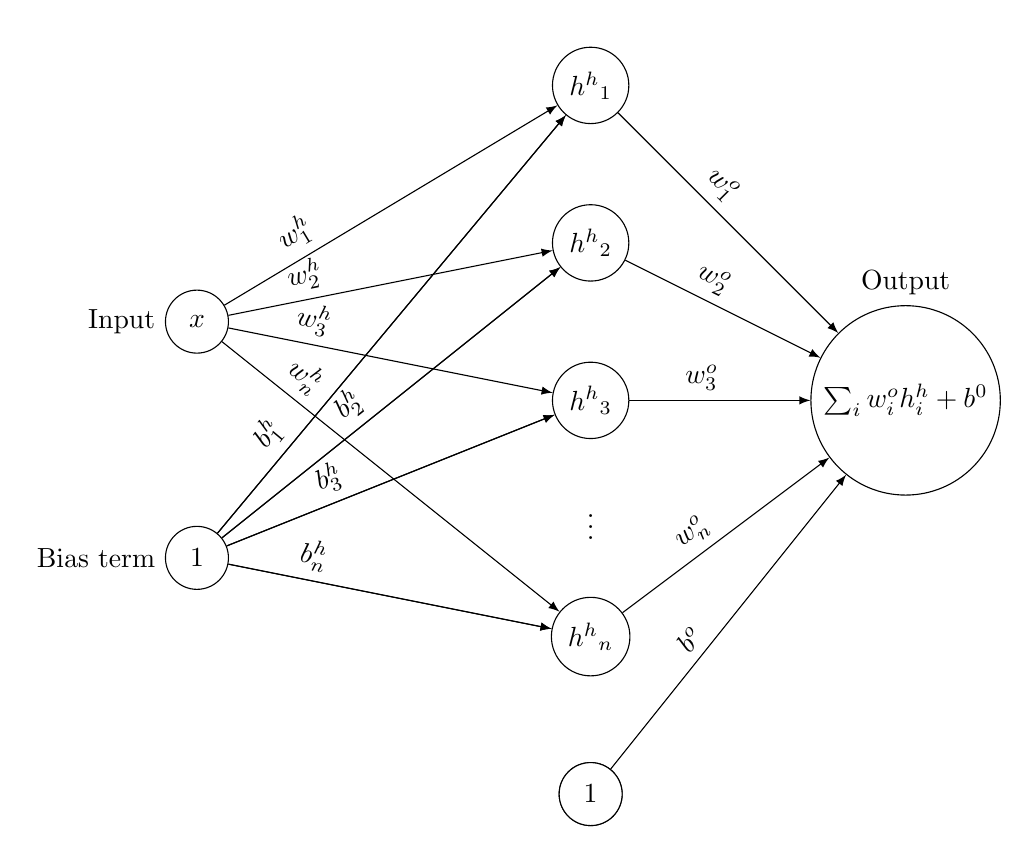
\begin{tikzpicture}
	[   cnode/.style={draw=black,draw=black,fill=#1,minimum width=8mm,circle},
	]
	\tikzset{normal arrow/.style={draw,-latex}}
	\node[cnode=white,label=90:Output] (s) at (9,-6) {$\sum_{i} w^o_{i} h^h_i + b^0$};
	\node[cnode=white,label=180:Bias term] (x-2) at (0,-8) {1};
	\node[cnode=white,label=180:] (p-5) at (5,-11) {1};
	\node at (5,-7.5) {$\vdots$};
	
	\node[cnode=white,label=180:Input] (x-1) at (0,-5) {$x$};
	
	\foreach \x in {1,...,5}
	{
		\pgfmathparse{\x<4 ? \x : "n"}	   
		\ifnum \x = 4
		
		
		\node[cnode=white,label=90:] (p-\x) at (5,{-2.*\x-div(\x,4)}) {${h^h}_n$};
		
		\else
		
		\ifnum \x = 5
		
		
		\node[cnode=white,label=90:] (p-\x) at (5,{-2*\x-div(\x,4)}) {$ 1 $};
		
		\else
		
		\node[cnode=white,label=90:] (p-\x) at (5,{-2*\x-div(\x,4)}) {${h^h}_{\x}$};
		
		\fi
		
		
		\fi
		\ifnum \x = 5
		\path[normal arrow] (p-\x) -- node[above,sloped,pos=0.4] {$b^{o}$} (s);
		\else
		\path[normal arrow] (p-\x) -- node[above,sloped,pos=0.4] {$w^o_{\pgfmathresult}$} (s);
		\fi
	}
	
	
	\foreach \x in {1,...,2}
	{   
		\foreach \y in {1,...,4}
		{   
			\ifnum \x=1
			\ifnum \y=4
			\path[normal arrow] (x-\x) -- (p-\y) node[above,sloped,pos=0.2] {$w^h_{n}$};
			
			\else
			\ifnum \y=5
			\path[normal arrow] (x-\x) -- (p-\y) node[below,sloped,pos=0.15] {$w_{w n+1}$};
			\else 
			\path[normal arrow] (x-\x) -- (p-\y) node[above,sloped,pos=0.25] {$w^h_{\y}$};
			
			\fi
			\fi
			\else
			\path[normal arrow] (x-\x) -- (p-\y); 		
			\fi
			
			\ifnum \x=2
			\ifnum \y=4
			\path[normal arrow] (x-\x) -- (p-\y) node[above,sloped,pos=0.25] {$b^h_{n}$};
			\else
			\ifnum \y=2
			\path[normal arrow] (x-\x) -- (p-\y) node[above,sloped,pos=0.42] {$b^h_{\y}$};
			\else
			\ifnum \y=3
			\path[normal arrow] (x-\x) -- (p-\y) node[above,sloped,pos=0.34] {$b^h_{\y}$};
			
			\else
			
			\path[normal arrow] (x-\x) -- (p-\y) node[above,sloped,pos=0.2] {$b^h_{\y}$};
			\fi
			\fi
			\fi
			\fi
			%\draw (x-\x) -- (p-\y) node[above,sloped,pos=0.3] {$\omega_{\x\y}$};
		}
	}
	\end{tikzpicture}
	
\end{center}

Według uniwersalnego twierdzenia aproksymacyjnego jednokierunkowa sieć neuronowa z jedną warstwą ukrytą i skończoną ale wystarczająco dużą liczbą neuronów, może przybliżyć z dowolną dokładnością każdą funkcję.

W 1989 roku Cybenko [cytowanie] udowodnił uniwersalne twierdzenie aproksymacyjne dla jednokierunkowej sieci neuronowej z sigmoidalną funkcją aktywacji. Jeszcze w tym samym roku, po pracy Cybenki ukazała się praca Hornika, Stinchcombe'a and White'a, którzy udowodnili prawdziwość powyższego twierdzenia dla dowolnej funkcji aktywacji.

Funkcje sigmoidalne to rodzina funkcji szeroko stosowanych w jednokierunkowych sieciach neuronowych, szczególnie tych stworzonych do celów regresji. W tej części zaprezentuję dowód uniwersalnego twierdzenia aproksymacyjnego podany przez Cybenkę w 1989 roku, następnie zademonstruję dowód wizualny posługując się sigmoidą jako funkcją aktywacji.



Niech $I_n$ oznacza $n$-wymiarową jednostkową kostkę , $[0,1]^n$. $C(I_n)$ to przestrzeń ciągłych funkjci na $I_n$. Dodatkowo, niech $M(I_n)$ oznacza przestrzeń skończonych, regularnych miar borelowskich na $n$-wymiarowej kostce jednostkowej $I_n$.

\begin{definition}
	Miara $\mu$ jest regularna jeśli dla każdego mierzelnego zbioru $A$, $\mu(A)$ równa się supremum miar zamkniętych podzbiorów $A$ i infimum otwartych nadzbiorów $A$. [Probability measures on metric spaces K.R. Parthasarathy]	
\end{definition}


%\begin{definition} Zobaczymy czy się przyda
%	$f:I_n \rightarrow C(I_n),$
%	$||f|| = \sup {|f(x)| : x \in I_n }$.
%\end{definition}
% 
% 
% $||f||$ is used to denote the supremum norm of an $f \in C(I_n)$. 

\begin{definition}
	Funkcja $\sigma: \mathbb{R} \rightarrow \mathbb{R}$ jest funkcją sigmoidalną jeśli
	\begin{eqnarray*}
		\sigma(x) \rightarrow \begin{cases} 1 \;\;\;\text{as} &x \rightarrow +\infty\\ 0 \;\;\;\text{as} &x \rightarrow -\infty\end{cases}
	\end{eqnarray*}
	
\end{definition}



\begin{definition}
	Funkcja $\sigma$ jest funkcją dyskryminaczyjną jeśli dla miary $\mu \in M(I_n)$ zachodzi 
	
	\begin{equation}
	\int_{I_n} \sigma \left( w^\mathsf{T}x + b_0 \right) d\mu(x) = 0
	\end{equation}
	dla każdego $w\in \mathbb{R}$ i $b_0 \in \mathbb{R}$ co implikuje, że $\mu = 0$.
	
\end{definition}


\begin{theorem}
	Każda ograniczona, mierzalna funkcja sigmoidalna $\sigma$ jest funkcją dyskryminacyjną. W szczególności każda ciągła funkcja sigmoidalna jest dyskryminacyjna.
	[cytowanie Cybenko]
\end{theorem}

Dowód uniwesalnego twierdzenia aproksymacyjnego przy wykorzystaniu funkcji sigmoidalnych wymaga wprowadzenia kilku przydatnych definicji i twierdzeń. Pierwsze z nich to twierdzenie Hahna-Banacha, które formułuje możliwość rozszerzenia każdego ograniczonego funkcjonału liniowego z podprzestrzeni unormowanej na całą podprzestrzeń, przy zachowaniu jego właściwości.


\begin{theorem}[Twierdzenie Hahna-Banacha]
	
	
	Niech $X$ to rzeczywista przestrzeń wektorowa, $p$ to funkcja rzeczywista zdefiniowana na $X$ spełniająca
	
	$$	p \left(\alpha x + (1-\alpha) y \right) \leq \alpha p(x)  + (1 - \alpha)p(y) \;\;\;\;\;\; \forall \alpha \in \left[0,1\right], x, y \in X$$
	
	
	Przypuśmy, że $\lambda$ to funkcjonał liniowy zdefiniowany na zbiorze $Y\subset X $, który spełnia
	$$\lambda(x) \leq p(x) \;\;\;\;\;\; \forall x \in Y.$$
	
	
	Wtedy istnieje funkcjonał liniowy $\Lambda$ zdefiniowany na $X$ spełniający
	$$\Lambda(x) \leq p(x) \;\;\;\;\;\; \forall x \in X,$$
	
	tak, że
	
	$$\Lambda(x) = \lambda(x) \;\;\;\;\;\; \forall x \in Y.$$
	
	
	Reed \& Simon (1980), Methods of Modern Mathematical Physics. Functional Analysis
\end{theorem}


\begin{definition}	
	
	Przestrzeń $\mathcal{L}\left(\mathcal{H}, \mathbb{C}\right)$ nazywana jest przestrzenią dualną przestrzeni Hilberta $\mathcal{H}$ i oznaczamy ją przez $\mathcal{H^*}$. Elementy $\mathcal{H^*}$ nazywane są ciągłymi funkcjonałami liniowymi.
	
	
	Reed \& Simon (1980), Methods of Modern Mathematical Physics. Functional Analysis
	
\end{definition}	


Twierdzenie Riesza opisuje przestrzeń $\mathcal{H^*}$.  


\begin{theorem}[Twierdzenie Riesza (znaleźć polskie źródło)]
	
	Dla każdego $T \in \mathcal{H^*}$, istnieje unikalne $y_T \in \mathcal{H}$ takie, że $$T(x) = \langle y_T, x \rangle \;\;\;\;\;\; \forall x \in \mathcal{H} $$
	
	
	Ponadto $$||y_T ||_{\mathcal{H}}  = ||T||_{\mathcal{H^*}}$$
	
	Reed \& Simon (1980), Methods of Modern Mathematical Physics. Functional Analysis
	
\end{theorem}


\begin{theorem}[]
	
	Niech $\sigma$ będzie ciągłą funkcją dyskryminacyjną, wtedy skończona suma
	
	\begin{equation}
	G\left(x\right) = \sum_{i=1}^{N} w^{o}_i \sigma\left({w^h_i}^{\mathsf{T}}x + b^h_i\right)
	\end{equation}
	
	jest gęsta w $C(I_n)$. Innymi słowy, dla danej funkcji $f \in C(I_n)$ i $\epsilon >0$, istnieje suma
	
	$G(x)$ mająca powyższą postać, dla której
	
	$$
	|G(x) - f(x)| < \epsilon \;\;\;\;\;\;\;\; \forall x \in I_n
	$$
\end{theorem}

\begin{proof}
	
	
	Niech $S \subset C(I_n)$ będzie zbiorem funkcji w postaci $G(x)$ lub w innych słowach - zbiorem sieci neuronowych. Z pewnością $S$ jest podprzestrzenią liniową $C(I_n)$. Jeśli $S$ jest gęsty, domknięcie $S$ jest całą przestrzenią $C(I_n)$.
	
	Przyjmijmy, że domknięcie $S$ nie jest całą przestrzenią $C(I_n)$. Wtedy domknięcie $S$ -- $S'$ jest domkniętą podprzestrzenią $C(I_n)$. Przez twierdzenie Hahna-Banacha, istnieje ograniczony funkcjonał liniowy na $C(I_n)$, nazwijmy go $L$, z własnością, że $L \neq 0$ ale $L(S') = L(S) = 0$.
	
	Przez twierdzenie Riesza, ograniczony funkcjonał liniowy $L$ ma postać
	
	$$
	L(h) = \int_{I_n} h(x)d\mu(x)
	$$
	
	dla $\mu \in M(I_n)$, dla każdego $h \in C(I_n)$. W szczególności, odkąd $\sigma(w^\mathsf{T}x + b)$  $\in S'$ dla każdego $w$ i $b$, musi zachodzić
	
	$$
	\int_{I_n} \sigma \left(w^\mathsf{T}x + b \right) d\mu(x) = 0 
	$$
	
	Jednakże, założyliśmy, że $\sigma$ jest funkcją dyskryminacyjną, ten warunek implikuje, że $\mu = 0$ co jest sprzeczne z naszym założeniem. Stąd, podprzestrzeń $S$ jest gęsta w $C(I_n)$.
	
	Pokazuje to, że suma
	
	$$
	G\left(x\right) = \sum_{i=1}^{N} w^{o}_i \sigma\left({w^h_i}^{\mathsf{T}}x + b^h_i\right)
	$$
	
	jest gęsta w $C(I_n)$ pod warunkiem, że $\sigma$ jest ciągła i dyskryminacyjna.
	
	Z twierdzenia wynika, że każda sieć neuronowa o wystarczająco dużej liczbie neuronów w jednej warstwie ukrytej i sigmoidalną funkcją aktywacyjną może z dowolną dokładnością przybliżyć przebieg każdej funkcji.
	
\end{proof}



%\begin{table}
%		\begin{center}
%	\begin{tabular}{ | l | c | }
%		\hline
%		Number of hidden neurons & Mean squared error \\ \hline
%		1 & 0.00942516615858  \\ \hline
%		2 & 0.00277472585580  \\ \hline
%		3 & 0.00135999931016  \\ \hline
%		4 & 5.33546419190e-05  \\ \hline
%		10 & 1.70243920789e-06  \\ \hline
%		100 & 1.11243069317e-06  \\ \hline
%		\hline
%	\end{tabular}
%		\end{center}
%\end{table}







\subsubsection{Przedstawienie wizualne działania}



\begin{figure}[h!]
	\centering
	\includegraphics[width=\linewidth]{cybenko14_12_1}
	
\end{figure}

\begin{figure}[h!]
	\centering
	\includegraphics[width=\linewidth]{mse}
	
\end{figure}



\subsection{Problem Bias - Variance}

\newpage
\section{Metodologia analizy}
\subsection{Keras}
Modele sieci neuronowych opisywane w tej pracy zostały zaprogramowane przy użyciu biblioteki Keras. Keras jest interfejsem API wysokiego poziomu służącym do tworzenia i szkolenia modeli głębokiego uczenia. Początkowo Keras został opracowany dla naukowców, którzy mogli dzięki niemu dokonywać szybkich eksperymentów i symulacji. Dzięki temu, że jest rozpowszechniany pod licencją MIT, co oznacza, że może być za darmo wykorzystywany w projektach komercyjnych, zdobył dużą popularność. Dziś ma on kilka set tysięcy użytkowników, od nauczycieli akademickich po inżynierów oprogramowania pracujących zarówno w start-upach jak i dużych firmach, i hobbystów. Jego zalety są wykorzystywane między innymi w wiodących ośrodkach naukowych takich jak Europejska Organizacja Badań Jądrowych CERN i setkach firm, z których największe to Google, Netflix, Uber, Yelp, Opera Software. Kaggle to platforma internetowa, która organizuje konkursy na najlepsze modele służące do przewidywania i opisywania zbiorów danych przesyłanych przez firmy i użytkowników. Jednym z najpopularniejszych narzędzi wykorzystywanych przez analityków jest Keras, wiele z konkursów zostało wygranych przez modele zbudowane przy użyciu wspomnianego interfejsu API.

Do największych zalet Keras należą:
\begin{itemize}
	\setlength\itemsep{0.em}
	
	\item  posiada przyjazny użytkownikowi interfejs, który ułatwia szybkie prototypowanie modeli sieci neuronowych
	\item  prosty i spójny interfejs zoptymalizowany pod kątem typowych przepadków użycia
	\item  zapewnia przejrzyste informacje zwrotne dotyczące błędów użytkownika
	\item  obsługuje dowolne architektury sieciowe: modele z wieloma wejściami lub wieloma wyściami
	\item posiada wbudowane wsparcie dla splotowych sieci neuronowych oraz rekurencyjnych sieci neuronowych
	\item  pozwala na bezproblemowe działanie tego samego kodu na CPU oraz GPU
\end{itemize}


Keras jest biblioteką, o której można powiedzieć, że zapewnia cegły służące do zbudowania modelu głębokiego uczenia natomiast w minimalnym stopniu pozwala użytkownikom na ingerencję w ich strukturę. W zamian wykorzystuje wyspecjalizowaną i dobrze zoptymalizowaną bibliotekę wyspecjalizowaną w operacjach na tensorach. Szczególnie szybko wykonują się obliczenia numeryczne typowe dla algorytmów uczenia maszynowego takich jak mnożenie macierzy i obliczanie gradientu.  Można wybierać wśród trzech istniejących implementacji, każda z nich ma otwarte źródło. Pierwsza z nich wykorzystuje Tensorflow opracowany i rozwijany przez Google'a, druga korzysta z Theano opracowanego i rozwijanamegp przez LISA Lab w Uniwersytecie Montrealskim, ostatnia i najmniej popularna wykorzystuje CNTK opracowane i rozwijane przez Microsoft. W przyszłości prawdopodobnie pojawi się więcej możliwości wyboru, między innymi niedawno powstały, zdobywający coraz większą popularność projekt Torch finansowany przez Facebooka. Obecnie najczęściej wykorzystywany jest TensorFlow, został on także wykorzystany w tej pracy. 


Poniżej zaprezentuję jak proste jest zbudowanie i wytrenowanie bardzo podstawowego przykładu sieci neuronowej przy użyciu biblioteki Keras. Cały proces wymaga wykonania kilku kroków:
\begin{enumerate}
	\setlength\itemsep{0.em}
	\item Zdefiniuj swoje dane treningowe: dane wejściowe i dane wyjściowe
	\item Zdefiniuj warstwy swojej sieci neuronowej, które przekształcają dane wyjściowe w wyjście
	\item Skonfiguruj proces uczenia poprzez wybranie funkcji straty, algorytmu szukającego minimum funkcji straty
	\item Przeprowadź odpowiednią do wytrenowania sieci ilość iteracji
\end{enumerate}

Zdefiniowana poniżej sieć składa się z dwóch warstw ukrytych o odpowiednio 10 i 5 neuronach ukrytych. Funkcją aktywacji w pierwszej warstwie jest sigmoida, dane wejściowe zawierają dwie cechy, które posłużą do zbudowania modelu, druga warstwa wykorzystuje tangens hiperboliczny jako funkcję aktywacji. Model podczas nauki minimalizuje błąd średniokwadratowy, wykorzystuje do tego algorytm rmsprop, trenownanie modelu skończy się po 100 pełnych iteracjach zbioru danych.


\begin{lstlisting}
#Zaimportuj wymagane pliki
from keras import models
from keras import layers

#Zainicjalizuj model
model = models.Sequential()

#Dodaj pierwszą warstwę
model.add(layers.Dense(units = 10, activation = 'sigmoid', input_shape = 2))

#Dodaj drugą warstwę
model.add(layers.Dense(units = 5, activation = 'tanh'))

#Dodaj warstwę wyjsciową
model.add(layers.Dense(units = 1))

#Skompiluj model
model.compile(optimizer = 'rmsprop', loss='mse')

#Trenuj model
model.fit(inputs = X, outputs = Y, epochs = 100)
\end{lstlisting}

%Przepisz stronę 63 z przepisem na zbudowanie modelu.
%
%3.6.4 K-fold validation do  przepisania ;

%Deep Learning with Python Francois Chollet Manning Shelter Island 2018



\subsection{Dane wejściowe}

\subsection{Replikacja danych}

\subsection{Funkcja straty}
Czemu jest taka funkcja i skąd warunek na eta?

\begin{equation}
\chi^2 = \sum_{k=1}^{N_{\sigma}} \left[ \sum_{i=1}^{n_k} \left( \frac{\eta_k \sigma^{th}_{ki} - \sigma^{ex}_{ki}}{\Delta \sigma_{ki}} \right)^2 + \left(\frac{\eta_k - 1}{\eta_k}\right)^2 \right]
\end{equation}


\begin{equation}
\eta_k = \frac{\sum_{i=1}^{n_k}\frac{\sigma_{ki}^{th} \sigma_{ki}^{ex}}{\left(\Delta \sigma_{ki}\right)^2} + \frac{1}{\left(\Delta \eta_k\right)^2}}{\sum_{i=1}^{n_k}\frac{\left(\sigma_{ki}^{th}\right)^2}{\left(\Delta \sigma_{ki}\right)^2} + \frac{1}{\left(\Delta \eta_k\right)^2}}
\end{equation}

Kilka niezależnych paragrafów

\subsection{Walidacja krzyżowa}

Algorytm wykorzystywany podczas nauki modelu ma za zadnianie znalezienie takich parametrów, które sprawiają, że model odwzorowuje dane wykorzystane do nauki w sposób jak najlepszy z możliwych. Jeśli do walidacji modelu wykorzystamy inną, niezależną próbkę danych pochodzącą z tego samego zbioru co podzbiór uczący, zazwyczaj okaże się, że model nie działa aż tak dobrze jak przy użyciu zbioru uczącego. Rozmiar tej różnicy zwiększa się, szczególnie wtedy gdy wielkość zbioru treningowego jest niewielka, lub gdy liczba parametrów modelu jest bardzo duża.
Walidacja krzyżowa to metoda statystyczna, która ma za zadanie zminimalizować tę różnicę przez co pomaga ocenić i zwiększyć trafność przewidywań modelu predykcyjnego. 


W najprostszym przykładzie walidacji krzyżowej zbiór danych dzieli się na dwa podzbiory: uczący i walidacyjny. Podczas gdy zbiór uczący służy do nauki modelu, zbiór walidacyjny wykorzystuje się aby mierzyć błąd modelu na nieznanym zbiorze danych. 

W algorytmie $k$-krotnej walidacji krzyżowej zbiór danych jest losowo dzielony na $k$ równych wielkością podzbiorów. Jeden z $k$ podzbiorów jest przeznaczany na zbiór walidacyjny, pozostałe $k-1$ podzbiorów służą jako dane teningowe. Powyżej opisana procedura jest powtarzana $k$ razy, a każdy $k$ podzbiorów dokładnie raz zostaje wykorzystany jako zbiór testowy. Następnie $k$ wyników modelu jest uśrednianych dając w rezultacie jeden wynik. \figurename{} \ref{fig:cross-val} przedstawia sposób działania $10$-krotnej walidacji krzyżowej.

\begin{figure}[htp!]
	\centering
	\includegraphics[width=1\textwidth]{cross_val.png}
	\caption{Na podstawie [Python Machine Learning
		Book by Sebastian Raschka]}
	\label{fig:cross-val}
\end{figure}

Cytując [Page 184, An Introduction to Statistical Learning, 2013.], "(...) istnieje pewien kompromis między obciążeniem a wariancją, związany z wyborem parametru $k$ w $k$-krotnej walidacji krzyżowej. Zazwyczaj stosuje się wartości z przedziału od 5 do 10, ponieważ pokazano empirycznie, że w takim wypadku otrzymujemy przewidywania, które nie cierpią nadmiernie ani z powodu dużego obciążenia ani dużej wariancji." Podczas treningu modelu wybrano $k = 6$, wykorzystując fakt, że liczba próbek w zbiorze danych jest całkowicie podzielna przez tę liczbę co zapewnia równy rozmiar wszystkich zbiorów treningowych i walidacyjnych.

\subsection{Wczesne zatrzymanie}
Algorytmy uczenia maszynowego dopasowują parametry modelu na podstawie danych treningowych o skończonym rozmiarze. Podczas procesu szkolenia model jest oceniany na podstawie tego, jak dobrze przewiduje obserwacje zawarte w tym zbiorze. Jednak celem uczenia maszynowego jest stworzenie modelu, który ma zdolność do przewidywania uprzednio niewidzianych obserwacji. Nadmierne dopasowanie to zjawisko pojawiające się wtedy gdy model za bardzo dopasowuje się do danych w zbiorze uczącym co powoduje zmniejszenie wartości błędu na tym zbiorze lecz równocześnie jest przyczyną wzrostu błędu na zbiorze testowym. Nadmierne dopasowanie modelu to problem, który może się pojawiać gdy model zawiera więcej parametrów niż wymagałaby tego natura modelowanego zjawiska. Sieć neuronowa to struktura skłonna do przeuczania. Podczas gdy obserwowany błąd obliczany w oparciu o dane treningowe spada, w pewnym momencie wartość błędu dla zbioru walidacyjnego zaczyna wzrastać. \figurename{} \ref{fig:loss_curves} przedstawia często zamieszczane w literaturze, wyidealizowane krzywe zmiany wartości funkcji straty w czasie, dla zbiorów treningowego i walidacyjnego. Najlepszy model predykcyjny miałby parametry, które odpowiadają momentowi globalnego minimum dla zbioru walidacyjnego.


\begin{figure}[htp!]
	\centering
	\includegraphics[width=1\textwidth]{early_stopping14_8.png}
	\caption{Wyidealizowane przykłady krzywych przedstawiających zmianę wartości funkcji straty na zbiorach treningowym i walidacyjnym, podczas nauki modelu}
	\label{fig:loss_curves}
\end{figure}

W dziedzinie uczenia maszynowego, metoda wczesnego zatrzymania to forma regularyzacji, która pozwala uniknąć problemu przeuczenia, zatrzymując naukę modelu gdy wartość funkcji straty na zbiorze walidacyjnym zaczyna wzrastać. Rzeczywisty przebieg wartości funkcji straty ma wiele lokalnych minimów, dlatego na podstawie obserwacji krzywych uczenia dokonano wyboru kryteriów zatrzymania nauki modelu. 
Niech $\Theta_{wa}(t)$ to wartość funkcji straty na zbiorze walidacyjnym po $t$ epokach, $\Theta_{min}(t)$ to dotychczasowe minimum funkcji straty na zbiorze walidacyjnym po $t$ epokach, definiowane jako:
$$
\Theta_{min}(t) \equiv \min_{t' < t} \Theta_{wa}(t')
$$

Niech $\Theta_{sr}(t)$ będzię średnią wartością funkcji straty dla zbioru walidacyjnego z ostatnich 10 epok.

$$
\Theta_{sr}(t) \equiv \frac{1}{10} \sum_{i=0}^{10} \Theta_{wa}(t-i)
$$

Oraz zdefiniujmy pomocniczy parametr $GL(t)$


$$
GL(t) \equiv \frac{\Theta_{sr}(t)}{\Theta_{min}} - 1
$$


Podczas nauki przedstawioneg modelu, do wczesnego zatrzymania wystarczyło spełnienie jednego z dwóch obowiązujących warunków:

\begin{itemize}
	\item $\Theta_{min}(t) = \Theta_{min}(t+ 200)$ dla wszystkich $t \in [t,t+200]$, brak zmniejszenia minimalnej wartości funkcji straty dla zbioru walidacyjnego przez 200 epok 
	\item $ GL(t)  > 2$, względny wzrost średniej wartości funkcji straty przez ostatnie 10 epok względem osiągniętego minimum jest większy niż $200\%$
\end{itemize}

Po skończeniu nauki, wybierany jest model, który ma najmniejszą wartość funkcji straty na zbiorze testowym.

\subsection{Ilość neuronów}

Architektura sieci neuronowej, tzn. ilość warstw ukrytych oraz ilość neuronów w warstwach ukrytych jest zdeterminowana przez wymiar danych wejściowych, rodzaj rozwiązywanego problemu (klasyfikacja czy regresja) oraz relację między zmiennymi objaśniającymi i zmienną objaśnianą.

Uogólniony model liniowy przydatny w szerokim zakresie zastosowań, nie potrzebuję żadnej warstwy ukrytej. Bywa szczególnie przydatny gdy zbiór zawiera mało danych lub są one obarczone dużą niedokładnością. Nawet w przypadku gdy relacja między zmiennymi jest lekko nieliniowa, użycie prostego modelu liniowego może skutkować lepszym uogólnieniem problemu niż skomplikowany model będący wrażliwy na każdy szum znajdujący się w danych. Zgodnie z uniwersalnym twierdzeniem aproksymacyjnym jedna warstwa ukryta z wystarczająco dużą liczbą neuronów wystarcza aby z dowolną dokładnością dowolną ciągłą funkcję [cybenko]. Jeśli zmienna objaśniająca jest jednowymiarowa, wydaje się, że nie odniesiemy żadnej korzyści z skonstruowania sieci neuronowej o więcej niż jednej warstwie ukrytej. Sprawy komplikują się jednak gdy zmienna wejściowa jest dwu lub więcej wymiarowa. Dwuwarstowa sieć neuronowa zachowuje właściwości jednowarstwowej sieci neuronowej oraz osiąga zdolność nauki każdego problemu klasyfikacyjnego [1995 Bishop 123], ponadto wielowarstwowa sieć neuronowa z dwoma warstwami może skutkować dokładniejszymi wynikami wykorzystując mniejszą ilość parametrów niż jednowarstwowa sieć [Chester (1990)]. Na tej podstawie, do rozwiązania problemu regresji gdzie wejściem jest para liczb $(\varepsilon, Q^2)$ postanowiłem wybrać sieć neuronowa z dwoma warstwami ukrytymi. 


\begin{table}
	\centering
	
	\caption{Liczba parametrów sieci neuonowej z dwoma warstwami ukrytymi w zależności od liczby neuronów w warstwach}\label{tab:parameters_table} 
	
	
	\begin{tabular}{c|p{1cm}|p{1cm}|p{1cm}|p{1cm}}
		\backslashbox{I warstwa}{II warstwa} & 2 & 3 & 4 & 5\\\hline\hline
		2 & 14 & 18 & 22 & 26 \\ \hline
		3 & 19 & 24 & 29 & 34 \\ \hline
		4 & 24 & 30 & 36 & 42 \\ \hline
		5 & 29 & 36 & 43 & 50 \\ \hline
	\end{tabular}
\end{table}

Aby znaleźć odpowiednią liczbę neuronów w dwóch warstwach ukrytych, stworzyłem siatkę [2, 3, 4, 5] $\times$ [2, 3, 4, 5] neuronów i sprawdziłem, która konfiguracja daje najmniejszy błąd zbioru walidacyjnego. Dane zostały podzielone na zbiór treningowy i testowy w stosunku 2:1. Dla każdej konfiguracji wytrenowano 50 sieci i sprawdzono jak wygląda statystyka błędu. \tablename{} \ref{tab:parameters_table} zawiera porównanie liczby parametrów sieci neuronowej w zależności od liczby neuronów w warstwach ukrytych. Do eksperymentów wybrano konfiguracje charakteryzujące się rozsądną w porównaniu do rozmiaru danych wejsciowych liczbą parametrów. \figurename{} \ref{fig:neurony} przedstawia rozkłady minimalnej wartości funkcji straty uzyskanej na danych walidacyjnych uzyskanej z 50 treningów sieci dla każdej konfiguracji ilości neuronów. Wykres pudełkowy to forma graficznej prezentacji rozkładu, która pozwala w łatwy sposób ukazać położenie, rozproszenie oraz kształt empirycznego rozkładu badanej cechy statystycznej. Konfiguracja 3 $\times$ 5 charakteryzuje się najniższą medianą wartości funkcji straty oraz małą liczbą wartości odstających. Ta obserwacja pozwoliła zdecydować, że liczby neuronów będą wynosiły 3 i 5 w odpowiednio pierwszej i drugiej warstwie ukrytej, co za tym idzie sieć będzie miała 36 parametrów.



%opisać liczbę parametrów + poniższy obrazek

\begin{figure}[htp!]
	\centering
	\includegraphics[width=1\textwidth]{neuronyy14_8.png}
	\caption{Wykresy pudełkowe przedstawiające rozkład wartości funkcji straty w zależności od ilości neuronów w pierwszej i drugiej warstwie ukrytej}
	\label{fig:neurony}
\end{figure}


\begin{SCfigure}
	\centering
	\resizebox{7.cm}{!}{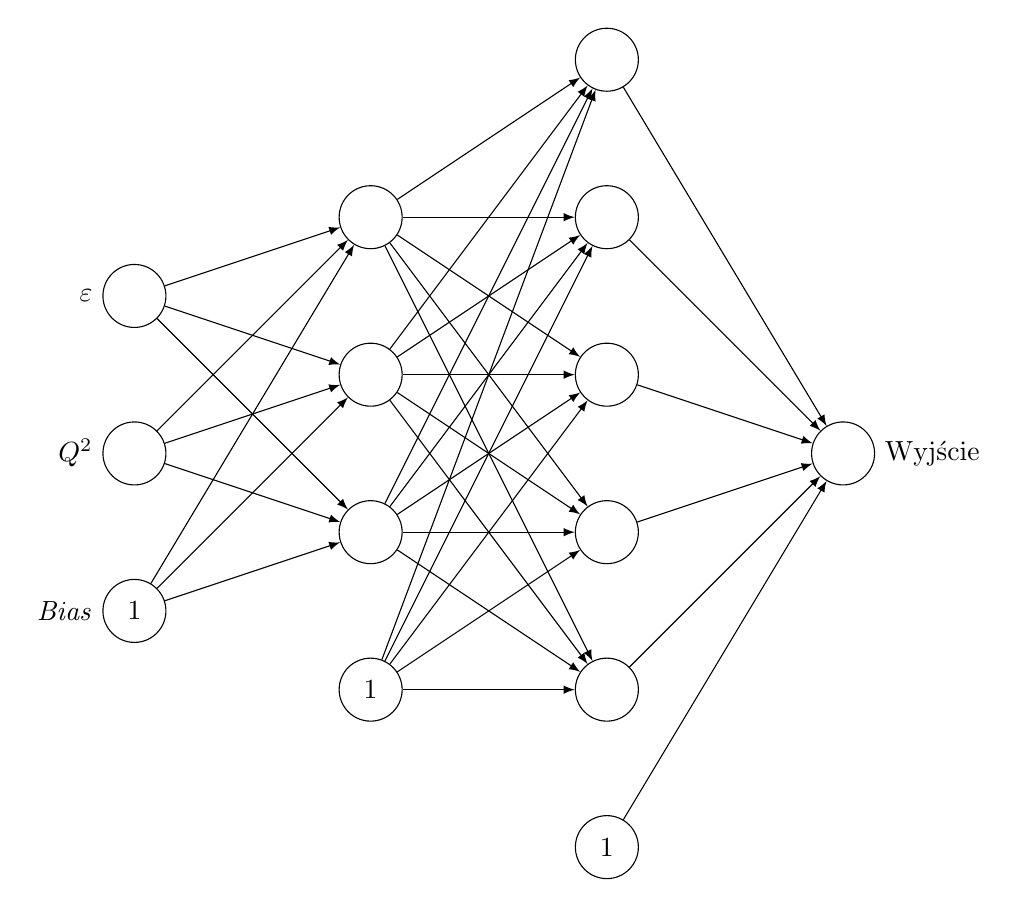
\begin{tikzpicture}
		[   cnode/.style={draw=black,draw=black,fill=#1,minimum width=8mm,circle},
		]
		\tikzset{normal arrow/.style={draw,-latex}}
		\node[cnode=white,label=0:Wyjście] (s) at (9,-7) {};
		
		\node[cnode=white,label=180:\textit{Bias}] (x-3) at (0,-9) {1};
		
		
		\node[cnode=white,label=180:] (p-4) at (3,-10) {$1$};
		
		\node[cnode=white,label=180:] (z-6) at (6,-12) {$1$};	
		
		
		\node[cnode=white,label=180:$\varepsilon$] (x-1) at (0,-5) {};
		\node[cnode=white,label=180:$Q^2$] (x-2) at (0,-7) {};
		
		\node[cnode=white,label=180:] (p-1) at (3,-4) {};
		\node[cnode=white,label=180:] (p-2) at (3,-6) {};
		\node[cnode=white,label=180:] (p-3) at (3,-8) {};
		
		\node[cnode=white,label=180:] (z-1) at (6,-2) {};
		\node[cnode=white,label=180:] (z-2) at (6,-4) {};
		\node[cnode=white,label=180:] (z-3) at (6,-6) {};
		\node[cnode=white,label=180:] (z-4) at (6,-8) {};
		\node[cnode=white,label=180:] (z-5) at (6,-10) {};
		
		
		
		\foreach \x in {1,...,6}
		{
			\path[normal arrow] (z-\x) -- node[above,sloped,pos=0.4] {} (s);
		}
		
		
		\foreach \x in {1,...,3}
		{   
			\foreach \y in {1,...,3}
			{   
				
				\path[normal arrow] (x-\x) -- (p-\y); 				
			}
		}
		
		\foreach \x in {1,...,4}
		{   
			\foreach \y in {1,...,5}
			{   
				
				\path[normal arrow] (p-\x) -- (z-\y); 
			}
			
			\ifnum \x=5
			\path[normal arrow] (z-\x) -- node[above,sloped,pos=0.4] {} (s);
			\else
			
			\fi
		}
		\end{tikzpicture}}
	\caption{Schemat zastosowanej sieci neuronowej, która składa się z: i) warstwy wejściowej z dwoma neuronami, ii) dwóch warstw ukrytych z odpowiednio trzema i pięcioma neuronami, iii) warstwy wyjściowej z jednym neuronem. Linie zakończone strzałką oznaczają wagę odpowiadającą każdej z par neuronów} \label{tab:scheme} 	
\end{SCfigure}

\subsection{Algorytm uczący}


Bardzo istotnym elementem tworzonego modelu jest wybór algorytmu poszukującego minimum funkcji straty oznaczonej na potrzeby tego paragrafu jako $J(\theta)$. Na podstawie jego wyników aktualizowane będą parametry tworzonej sieci neuronowej. Bardzo pomocną koncepcją pozwalającą zrozumieć istotę trudności problemu jest powierzchnia błędu "\textit{Każda z N wag i wartości progowych sieci (tzn. wszystkie wolne parametry modelu) traktowana jest jako jeden z wymiarów przestrzeni. W ten sposób każdy stan sieci, wyznaczony przez aktualne wartości jej N parametrów może być traktowany jako punkt na N-wymiarowej hiperpłaszczyźnie. N+1 wymiarem (zaznaczanym jako wysokość ponad wspomnianą wyżej hiperpowierzchnią) jest błąd, jaki popełnia sieć. Dla każdego możliwego zestawu wag i progów może więc zostać narysowany punkt w przestrzeni N+1 wymiarowej, w taki sposób, że stan sieci wynikający z aktualnego zestawu jej parametrów lokuje ten punkt na wspomnianej wyżej N-wymiarowej hiperpłaszczyźnie zaś wartość błędu, jaki popełnia sieć dla tych właśnie wartości parametrów stanowi wysokość umieszczenia punktu ponad tą płaszczyzną. Gdybyśmy opisaną procedurę powtórzyli dla wszystkich możliwych wartości kombinacji wag i progów sieci, wówczas otrzymalibyśmy "chmurę" punktów rozciągających się ponad wszystkimi punktami N-wymiarowej hiperpłaszczyzny parametrów sieci, tworzącą właśnie rozważaną powierzchnię błędu. Celem uczenia sieci jest znalezienie na tej wielowymiarowej powierzchni punktu o najmniejszej wysokości, czyli ustalenie takiego zestawu wag i progów, który odpowiada najmniejszej wartości błędu.
	Przy stosowaniu modeli liniowych z funkcją błędu opartą na sumie kwadratów powierzchnia błędu ma kształt paraboloidy (funkcji kwadratowej), ma więc kształt kielicha o gładkich powierzchniach bocznych i o jednym wyraźnym minimum. Z tego powodu wyznaczenie w tym przypadku wartości minimalnej nie stwarza większych problemów.}"[$https://www.statsoft.pl/textbook/stathome_stat.html?$]

Jeżeli dysponujemy niewielkim zbiorem danych treningowych, do znalezienia optimum funkcji doskonale sprawdzą się metody quasi-Newtonowskie. Ich zaletą jest bardzo szybka zbieżność, niestety obliczenie hesjanu funkcji wielu zmiennych charakteryzuje się dużą złożonością pamięciową $O(n^2)$ i jeszcze większą złożonością obliczeniową $O(n^3)$. Z tego powodu możliwość ich zastosowania ogranicza się do niewielu przypadków. Najbardziej znane algorytmy quasi-Newtonowskie to m.in: \textit{LM-BFGS, Levenberg-Marquardt.} Dysponując dużym zbiorem danych należy wybrać inny algorytm. Po za losowym poszukiwaniem parametrów, najłatwiejszym z nich i bardzo intuicyjnym jest metoda gradientu prostego (\textit{gradient descent}). Parametry $\theta$ aktualizowane są w następujący sposób:


\begin{equation}
\theta^{k+1} = \theta^{k} - \alpha \nabla J(\theta^{k})
\end{equation}


gdzie $\alpha$ to wybrany odpowiednio parametr szybkości uczenia (\textit{learning rate}) odpowiedzialny za stopień zmiany parametrów w kolejnych iteracjach. Jeśli $\theta^0$ znajduje się odpowiednio blisko minimum funkcji, i parametr $\alpha$ jest wystarczcająco niewielki, algorytm osiąga liniową zbieżność [Dennis, J., Schnabel, R.B.: Numerical Methods For Unconstrained Optimization and Nonlinear Equations. Prentice-Hall, Inc., Englewood Cliffs, New Jersey (1983)
]. W ogólności metoda gradientu prostego gwarantuje zbieżność do globalnego minimum w przypadku funkcji błędu o wypukłej powierzchni i do lokalnego minimum dla funkcji błędu o powierzchni nie wypukłej. Algorytm jednak jest bardzo wolny, co jest jego największą słabością. Ze względu na częstość aktualizacji wag, metodę gradientu prostego możemy podzielić na \textit{batch gradient descent} oraz \textit{stochastic gradient descent}. W pierwszym przypadku wagi są dostosowywane po przetworzeniu pełnego zbioru danych, w metodzie stochastycznej zbiór uczący dzielony jest na podzbiory a wagi aktualizowane są po przetworzeniu każdego z podzbiorów. Druga metoda jest szczególnie użyteczna dla dużych zbiorów danych. Spodziewamy się, że dla dobrze przygotowanych danych kierunek podążania wartości wag będzie podobny jeśli policzymy gradient zarówno dla 10\% jak i dla 100\% zbioru treningowego.


Wyobraźmy sobie, że poszukiwanie minimum powierzchni błędu to przemierzanie przestrzeni pełnej dolin, pagórków, wąwozów. W kolejnych iteracjach przeskakujemy między tymi obszarami, w pewnym momencie może się zdarzyć, że gradient zaniknie lub będzie bardzo słaby a nasze poszukiwania zatrzymają się nie osiągając wystarczającego minimum. Idea pędu inspirowana zjawiskami fizycznymi to nadanie gradientowi krótkotrwałej pamięci. Posługując się kolejną analogią, popchnięta w dół piłka nabierając prędkości zwiększa swój pęd. To samo dzieje się z parametrami sieci, wartość pędu wzrasta dla wymiarów, których gradienty wskazują te same kierunki i zmniejsza modyfikacje wartości dla wymiarów, w których gradienty zmieniają kierunki. W rezultacje otrzymujemy szybszą zbieżność i mniejsze oscylacje.

\begin{align} 
v^{k+1} &=  \beta v^{k}+ \nabla J(\theta^{k}) \\[0.4em]
\theta^{k+1} &=  \theta^{k }- \alpha v^{k+1}
\end{align}

Zmiana jest niewielka, gdy $\beta = 0$, otrzymujemy zwykłą metodę gradientu prostego, zazwyczaj jednak ustala się wartość parametru $\beta$, zwanego pędem na około $0.9$. [1986 Nature, Learning representations by back-propagating errors
David E. Rumelhart, Geoffrey E. Hinton \& Ronald J. Williams] 

\begin{figure}[h	]
	\centering
	\includegraphics[width=1\textwidth]{gd_sgd.png}
	\caption{Funkcja  $f(x,y) =(1.5 - x + xy)^2 + (2.25 - x + xy^2)^2 + (2.625 - x + xy^3)^2$, osiąga minimum równe 0, w punkcie $(3,0.5)$ oznaczonym  czarną gwiazdą. Grafika przedstawia porównanie działania metody gradientu prostego oraz jego modyfikacji poprzez dodanie pędu. Przyjmując, że punkt początkowy to $(2,1)$, $\alpha = 0.001$ i $\beta = 0.9$, możemy prześledzić trajektorie algorytmów przez pierwsze 500 iteracji działania.} 
	\label{fig:gd_sgd}
\end{figure}

Porównanie efektywności przedstawionych wyżej algorytmów znajduje się na \figurename{} \ref{fig:gd_sgd}, w zaprezentowanym przykładzie metoda gradientu prostego potrzebuje około 10 razy więcej iteracji od modyfikacji z pędem aby dotrzeć do minimum zaprezentowanej funkcji. Jest to przykład świadczący o tym jak duży wpływ na szybkość działania algorytmu wywiera ta niewieka modyfikacja. 


Wykorzystany podczas treningu modelu algorytm korzysta jednak z jeszcze z jednej modyfikacji. Nie chcielibyśmy aby piłka spuszczona w dół ślepo podążała za zboczem widząc, że za niedługo mocno się ono podniesie. Przyspieszenie Nesterova (\textit{NAG}) jest sposobem na uwzględnienie podczas obliczania gradientu przybliżonej przyszłej pozycji parametrów sieci.	

\begin{align} 
v^{k+1} &=  \beta v^{k}+ \nabla J(\theta^{k} - \beta v^{k}) \\[0.4em]
\theta^{k+1} &=  \theta^{k }- \alpha v^{k+1}
\end{align}
[https://arxiv.org/abs/1609.04747]


Niezywkle istotnym parametrem algorytmu jest $\alpha$, jego niezmienność wraz z postępem iteracji powoduje bardzo niską efektywność algorytmu. Ze względu na metodę zmiany tego parametru, który może być indywidualnie ustalany dla każdej wagi powstało wiele szeroko wykorzystywanych algorytmów. Do najpopularniejszych należą między innymi \textit{Adam, Nadam, Adagrad, Adadelta, AMSGrad, RMSprop}. 

W swoim algorytmie postanowiłem dokonywać zmiany parametru $\alpha$ wraz ze wzrostem iteracji. Ponadto szybkość uczenia zależna jest od wybranego parametru $\lambda$ decydującego o tym z jaką szybkością maleje.

\begin{equation}
\alpha(i) = \alpha_0 \times \frac{1}{1 + \lambda \times i}
\end{equation}

\figurename{} \ref{fig:hyperparameters} przedstawia porównanie przykładowych krzywych zmian wartości funkcji straty w czasie dla różnych wartości $\alpha$ i $\lambda$. Na ich podstawie widać jak duży wpływ wnosi parametr $\alpha$ w proces nauki modelu. Zbyt duża szybkość uczenia powoduje bardzo duże oscylacje krzywej funkcji straty, za mała wartość $\alpha$ bardzo mocno spowalnia proces nauki. Pewien kompromis przynosi wybranie odpowiednio dużej początkowej wartości szybkości uczenia, co przynosi szybkie przejście algorytmu w obszar minimum i następnie zmniejszenie go do wartości potrafiącej efektywnie dalej poszukiwać optimum. Zadowalający przebieg mają krzywe o parametrach $\alpha = 0.005$, $\lambda = 0.001$, które przedstawiają porządany, eksponencjalny kształt o niewielkiej oscylacji. Na podstawie powyższej analizy to właśnie te hiperparametry zostały wykorzystane w modelu, dodatkowo parametr pędu $\beta$ został ustalony na wartość $0.9$


\begin{figure}[htp!]
	\centering
	\includegraphics[width=1\textwidth]{hyperparameter14_16a.png}
	\caption{Porównanie przykładowych krzywych zmiany wartości funkcji straty w czasie dla zbiorów treningowego (kolor pomarańczowy) i walidacyjnego (kolor niebieski) ze względu na parametry $\alpha$ (\textit{learning rate}) oraz $\lambda$ (\textit{decay})}
	\label{fig:hyperparameters}
\end{figure}

\newpage

\section{Wyniki analizy}
\subsection{}

\end{document}
